\documentclass[border=6pt]{standalone}
% Shared preamble for web figures.  Each figure is a standalone .tex that
% \input's this file; scripts/make-figures.sh turns it into an SVG.
% Handouts pull the same file with \fig{Unit_X/<name>}.
\usepackage[T1]{fontenc}
\usepackage{helvet}
\renewcommand{\familydefault}{\sfdefault}
\renewcommand{\ttdefault}{pcr}  % Courier: a real Type 1 typewriter font
\usepackage{amsmath}
\usepackage{tikz}
\usetikzlibrary{arrows.meta,positioning,calc,shapes.symbols,shapes.geometric}

% Who makes the rules is the point of most diagrams in this book, so the
% colors mean the same thing everywhere: blue is a person, orange is the
% computer, green is an answer, pink is the human brain.
\definecolor{person}{HTML}{2C6FAE}
\definecolor{machine}{HTML}{D35400}
\definecolor{result}{HTML}{1E8449}
\definecolor{brainpink}{HTML}{C2185B}
\definecolor{ink}{HTML}{2C3E50}

\tikzset{
  doodle/.style={line width=1.5pt, line cap=round, line join=round, draw=ink},
  box/.style={draw, rounded corners=5pt, line width=1.1pt, align=center,
              inner sep=7pt, minimum height=1.0cm, font=\small},
  personbox/.style={box, draw=person, fill=person!10},
  machinebox/.style={box, draw=machine, fill=machine!10},
  resultbox/.style={box, draw=result, fill=result!10},
  plainbox/.style={box, draw=ink!70, fill=ink!4},
  flow/.style={-{Stealth[length=8pt]}, line width=1.4pt, draw=ink},
}

% A person (blue) and a robot head (orange) as small icons.
% \personicon{x}{y}{scale}   \roboticon{x}{y}{scale}
\newcommand{\personicon}[3]{%
  \begin{scope}[shift={(#1,#2)}, scale=#3]
    \fill[person] (0,0.62) circle (0.28);
    \fill[person, rounded corners=6pt] (-0.42,-0.55) rectangle (0.42,0.28);
  \end{scope}}
\newcommand{\roboticon}[3]{%
  \begin{scope}[shift={(#1,#2)}, scale=#3]
    \draw[machine, line width=1.2pt] (0,0.5) -- (0,0.72);
    \fill[machine] (0,0.78) circle (0.08);
    \draw[machine, line width=1.4pt, fill=machine!12, rounded corners=4pt] (-0.5,-0.45) rectangle (0.5,0.5);
    \fill[ink] (-0.2,0.12) circle (0.08);
    \fill[ink] (0.2,0.12) circle (0.08);
    \draw[ink, line width=1pt] (-0.22,-0.22) -- (0.22,-0.22);
  \end{scope}}

\begin{document}
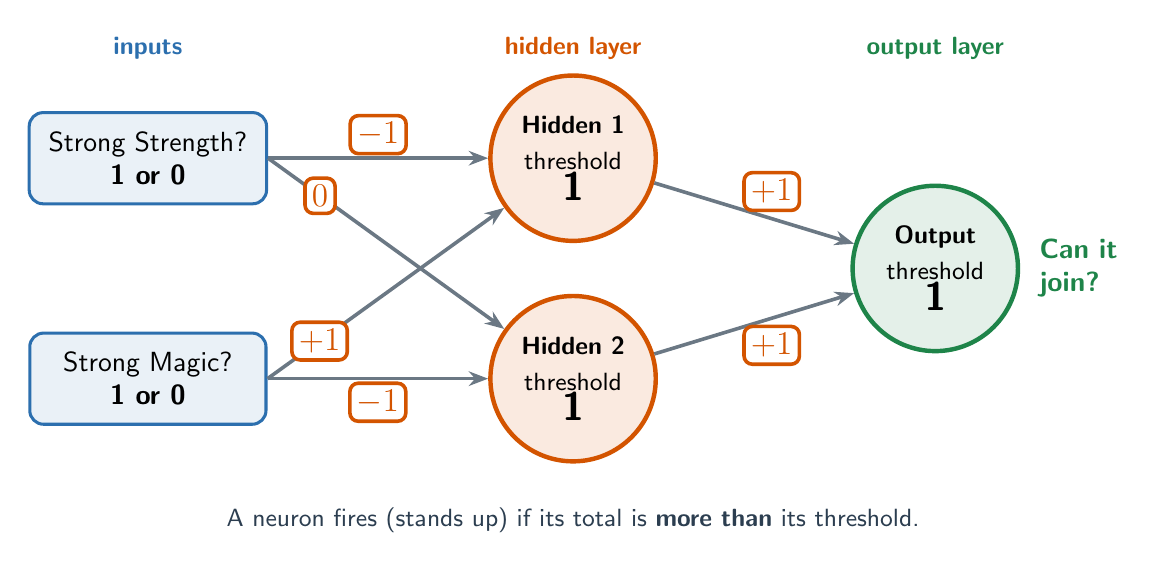
\begin{tikzpicture}[
  inp/.style={personbox, minimum width=3.0cm, font=\normalsize, align=center},
  neu/.style={circle, line width=1.6pt, minimum size=2.1cm, align=center, font=\small},
  wt/.style={fill=white, draw=machine, rounded corners=3pt, font=\large\bfseries, text=machine, inner sep=2.5pt},
  ln/.style={-{Stealth[length=7pt]}, line width=1.3pt, draw=ink!70},
]
% The class network for Lesson 2.5, with its starting numbers.
\node[inp] (s) at (0,2.6) {Strong Strength?\\\textbf{1 or 0}};
\node[inp] (m) at (0,-0.2) {Strong Magic?\\\textbf{1 or 0}};
\node[neu, draw=machine, fill=machine!12] (h1) at (5.4,2.6) {\textbf{Hidden 1}\\[2pt]threshold\\{\Large\bfseries 1}};
\node[neu, draw=machine, fill=machine!12] (h2) at (5.4,-0.2) {\textbf{Hidden 2}\\[2pt]threshold\\{\Large\bfseries 1}};
\node[neu, draw=result, fill=result!12] (o) at (10.0,1.2) {\textbf{Output}\\[2pt]threshold\\{\Large\bfseries 1}};
\node[font=\normalsize\bfseries, text=result, anchor=west, align=left] at (11.2,1.2) {Can it\\join?};
\draw[ln] (s.east) -- node[wt, pos=0.5, above=1pt] {$-1$} (h1);
\draw[ln] (s.east) -- node[wt, pos=0.22] {$0$} (h2);
\draw[ln] (m.east) -- node[wt, pos=0.22] {$+1$} (h1);
\draw[ln] (m.east) -- node[wt, pos=0.5, below=1pt] {$-1$} (h2);
\draw[ln] (h1) -- node[wt, pos=0.45, above right=-1pt] {$+1$} (o);
\draw[ln] (h2) -- node[wt, pos=0.45, below right=-1pt] {$+1$} (o);
\node[font=\small\bfseries, text=person] at (0,4.0) {inputs};
\node[font=\small\bfseries, text=machine] at (5.4,4.0) {hidden layer};
\node[font=\small\bfseries, text=result] at (10.0,4.0) {output layer};
\node[font=\small, text=ink, align=center] at (5.4,-2.0) {A neuron fires (stands up) if its total is \textbf{more than} its threshold.};
\end{tikzpicture}
\end{document}
